\chapter{Progetto di \textit{stage}}
    \section{Gestione degli \textit{stage} in SogeaSoft S.r.l.}
    SogeaSoft S.r.l. riconosce il valore strategico degli \textit{stage} curricolari, considerandoli un'opportunità sia per la formazione di potenziali nuovi dipendenti, sia per l'esplorazione di nuove tecnologie e la valutazione critica dei sistemi attualmente in uso. Tali percorsi formativi consentono non solo di trasferire conoscenze e competenze, ma anche di promuovere un'analisi approfondita delle soluzioni tecnologiche adottate dall'azienda, favorendo l'innovazione e l'ottimizzazione dei processi.  

    \vspace{0.2 em}
    \noindent Le attività svolte nell'ambito degli \textit{stage} possono includere: 
    \begin{itemize}
        \item l'integrazione di nuove funzionalità nei sistemi esistenti, con l'obiettivo di migliorarne le prestazioni e l'efficienza;
        \item lo studio e lo sviluppo di strumenti autonomi a supporto dei processi di sviluppo o dei prodotti in uso, come ad esempio Swagger, una piattaforma per la documentazione e il testing delle API (approfondite nella Sezione 1.7);  
        \item l'analisi formale di strumenti già utilizzati in azienda, ma impiegati prevalentemente in modo empirico, al fine di standardizzarne e ottimizzarne l’uso;  
        \item la conduzione di attività di monitoraggio sulle \textit{performance} di determinati sistemi, per identificarne eventuali criticità e proporre soluzioni migliorative.  
    \end{itemize}

    \vspace{0.2 em}
    \noindent L'evoluzione tecnologica in SogeaSoft S.r.l. può avvenire attraverso diverse strategie, tra cui l’ampliamento delle funzionalità della \textit{codebase} esistente, l’analisi teorica dello stato dell’arte o la realizzazione di \textit{software} sperimentali, quali \textit{Proof of $Concept_G$} ($PoC_G$) o prodotti già pronti per un utilizzo immediato, come il \textit{Minimum Viable $Product_G$} ($MVP_G$). Nel contesto del mio \textit{stage}, le attività svolte hanno combinato questi approcci, consentendo lo sviluppo di una soluzione concreta ma non immediatamente utilizzabile (ossia un \text{prototipo\textsubscript{G}}, la cui differenza è visualizzabile nella Figura 2.2); nonché la produzione di una documentazione tecnica approfondita. Tale metodologia si è rivelata particolarmente efficace per garantire una comprensione strutturata del problema e facilitare eventuali iterazioni successive.  
    \begin{figure}[H]
        \centering
        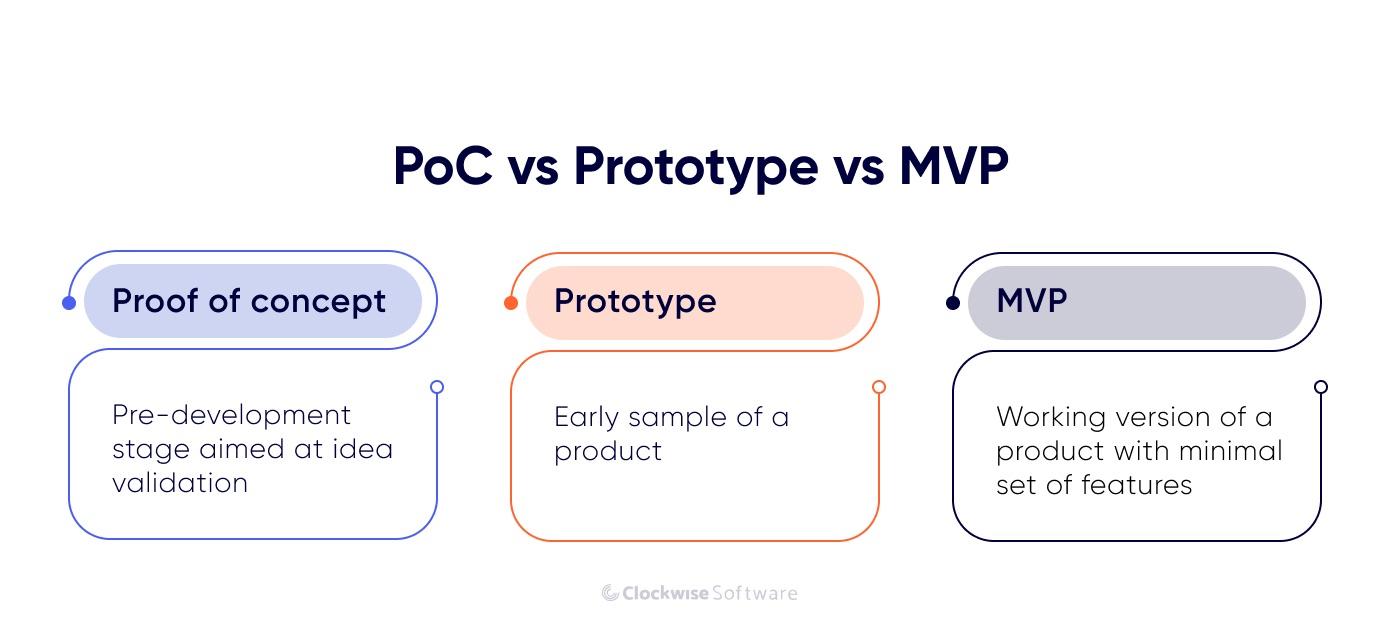
\includegraphics[width=0.5\linewidth]{BCS-Tessi/images/PoC_MVP.jpeg}
        \caption[Differenza tra PoC, Prototipo, MVP]{Differenza tra PoC, Prototipo, MVP. Fonte: https://clockwise.software/blog/proof-of-concept-in-software-development/ \textit{(ultimo accesso 12/03/2025)}}
        \label{fig:PoC-prototipo-MVP}
    \end{figure}

    \vspace{0.2 em}
    \noindent SogeaSoft S.r.l. attribuisce particolare valore agli \textit{stage}, poiché rappresentano un'opportunità strategica per affrontare una delle sue principali sfide tecnologiche: la migrazione del proprio prodotto da un’architettura $monolitica_G$ a un’architettura a $microservizi_G$, come discusso nella Sezione 1.8. Gli \textit{stage} costituiscono una risorsa vantaggiosa sotto molteplici aspetti: da un lato, permettono di ottimizzare l’investimento in ricerca e sviluppo grazie a costi contenuti; dall’altro, consentono all’azienda di entrare in contatto con prospettive innovative, idee originali e persone non condizionate dai paradigmi consolidati all'interno dell’azienda.  

    \vspace{0.2 em}
    \noindent Un ulteriore fattore determinante nell’impiego di tirocinanti per lo sviluppo di soluzioni innovative è la gestione delle risorse interne. Il personale aziendale è prevalentemente impegnato nel mantenimento e nell’evoluzione dei sistemi attualmente in produzione, rendendo complesso il reindirizzamento delle competenze su progetti sperimentali. L’inserimento di studenti permette di destinare risorse dedicate a iniziative di ricerca e innovazione, garantendo al contempo un processo di trasferimento di conoscenze tra le diverse generazioni di sviluppatori.
    
    \section{Il \textit{software} SAI}
    
    Il tema principale del mio \textit{stage} ha riguardato lo sviluppo e l’evoluzione di SAIonWeb, un \textit{software} basato sul \textit{framework} SAI (Sistema Aziendale Integrato). SAIonWeb è uno strumento progettato per la gestione dei processi aziendali nell’ambito dell’\textit{Enterprise Resource Planning} (ERP). In particolare, il \textit{software} è destinato al settore manifatturiero, con un \textit{focus} specifico sull'industria dell’abbigliamento, supportando l'intero ciclo di vita del prodotto: dalla gestione delle materie prime, alla fase di confezionamento, fino alla distribuzione finale\footnote{Fonte: https://sogeasoft.com/p/sai \textit{(ultima visita 12/03/2025)}}. 

    \vspace{0.2 em}
    \noindent Il \textit{framework} SAI, alla base di SAIonWeb, è caratterizzato da un'architettura monolitica, un modello in cui tutti i componenti del sistema, dall’interfaccia utente alla logica applicativa e alla gestione dei dati, sono strettamente integrati all’interno di un'unica applicazione\footnote{S. Newman, Monolith to Microservices: Evolutionary Patterns to Transform Your Monolith, O'Reilly Media, 2019.}.  

    \vspace{0.2 em}
    \noindent L'obiettivo del mio stage è stato analizzare il funzionamento di SAI, identificando il dominio applicativo, i \textit{bounded $contexts_G$} e le possibili suddivisioni in microservizi. Il lavoro ha comportato un'attività di studio approfondita dell'architettura esistente, al fine di individuare i servizi che potevano essere estratti e trasformati in unità indipendenti, contribuendo così al processo di migrazione verso SAIonWeb, pensata per adottare un'architettura a microservizi. Inoltre, il progetto ha previsto la valutazione delle scelte progettuali già adottate dai dipendenti, con la possibilità di proseguire il lavoro esistente o, ove necessario, modificarlo per garantire una transizione più efficace e coerente con i principi del \textit{Domain-Driven $Design_G$} (DDD). 
    
        \subsection{Funzionalità generali di SAI}
        SAI \textit{Enterprise Resource Planning} (ERP) è un sistema \textit{software} gestionale progettato per integrare e automatizzare i processi aziendali, consentendo alle organizzazioni di gestire in modo efficiente risorse, dati e operazioni. Questi sistemi offrono un ambiente centralizzato in cui le diverse aree aziendali – dalla produzione alla logistica, dalla contabilità alla gestione delle risorse umane – possono operare in modo coordinato, migliorando la tracciabilità delle informazioni e ottimizzando la produttività.  

        \vspace{0.2 em}
        \noindent SAI è un ERP specificamente sviluppato per il settore dell'abbigliamento, supportando l’intero ciclo di produzione e distribuzione di capi di moda. Le sue funzionalità principali includono:  
        \begin{itemize}
            \item \textbf{Gestione delle materie prime}: monitoraggio degli approvvigionamenti, delle scorte e della qualità dei materiali;
            \item \textbf{Pianificazione della produzione}: organizzazione delle fasi produttive, assegnazione delle risorse e gestione dei tempi di lavorazione;
            \item \textbf{Tracciabilità dei prodotti}: controllo dell’avanzamento di ciascun capo, dalla fase iniziale di lavorazione fino alla distribuzione. In particolare, una schermata d'esempio è visibile in Figura 2.1;
            \item \textbf{Gestione degli ordini e delle vendite}: registrazione degli ordini, gestione delle consegne e fatturazione automatizzata;
            \item \textbf{Logistica e distribuzione}: coordinamento delle spedizioni, gestione dei magazzini e ottimizzazione delle scorte;
            \item \textbf{Integrazione con il sistema contabile}: gestione di pagamenti, bilanci e rendicontazione finanziaria;
            \item \textbf{Monitoraggio delle performance aziendali}: generazione di \textit{report} analitici e strumenti di \textit{business intelligence} per supportare il processo decisionale.  
        \end{itemize}

        \vspace{0.2 em}
        \noindent Attraverso queste funzionalità, SAI consente alle aziende del settore moda di migliorare la gestione delle operazioni, ridurre i tempi di produzione e garantire una maggiore efficienza operativa.

        \begin{figure}[H]
            \centering
            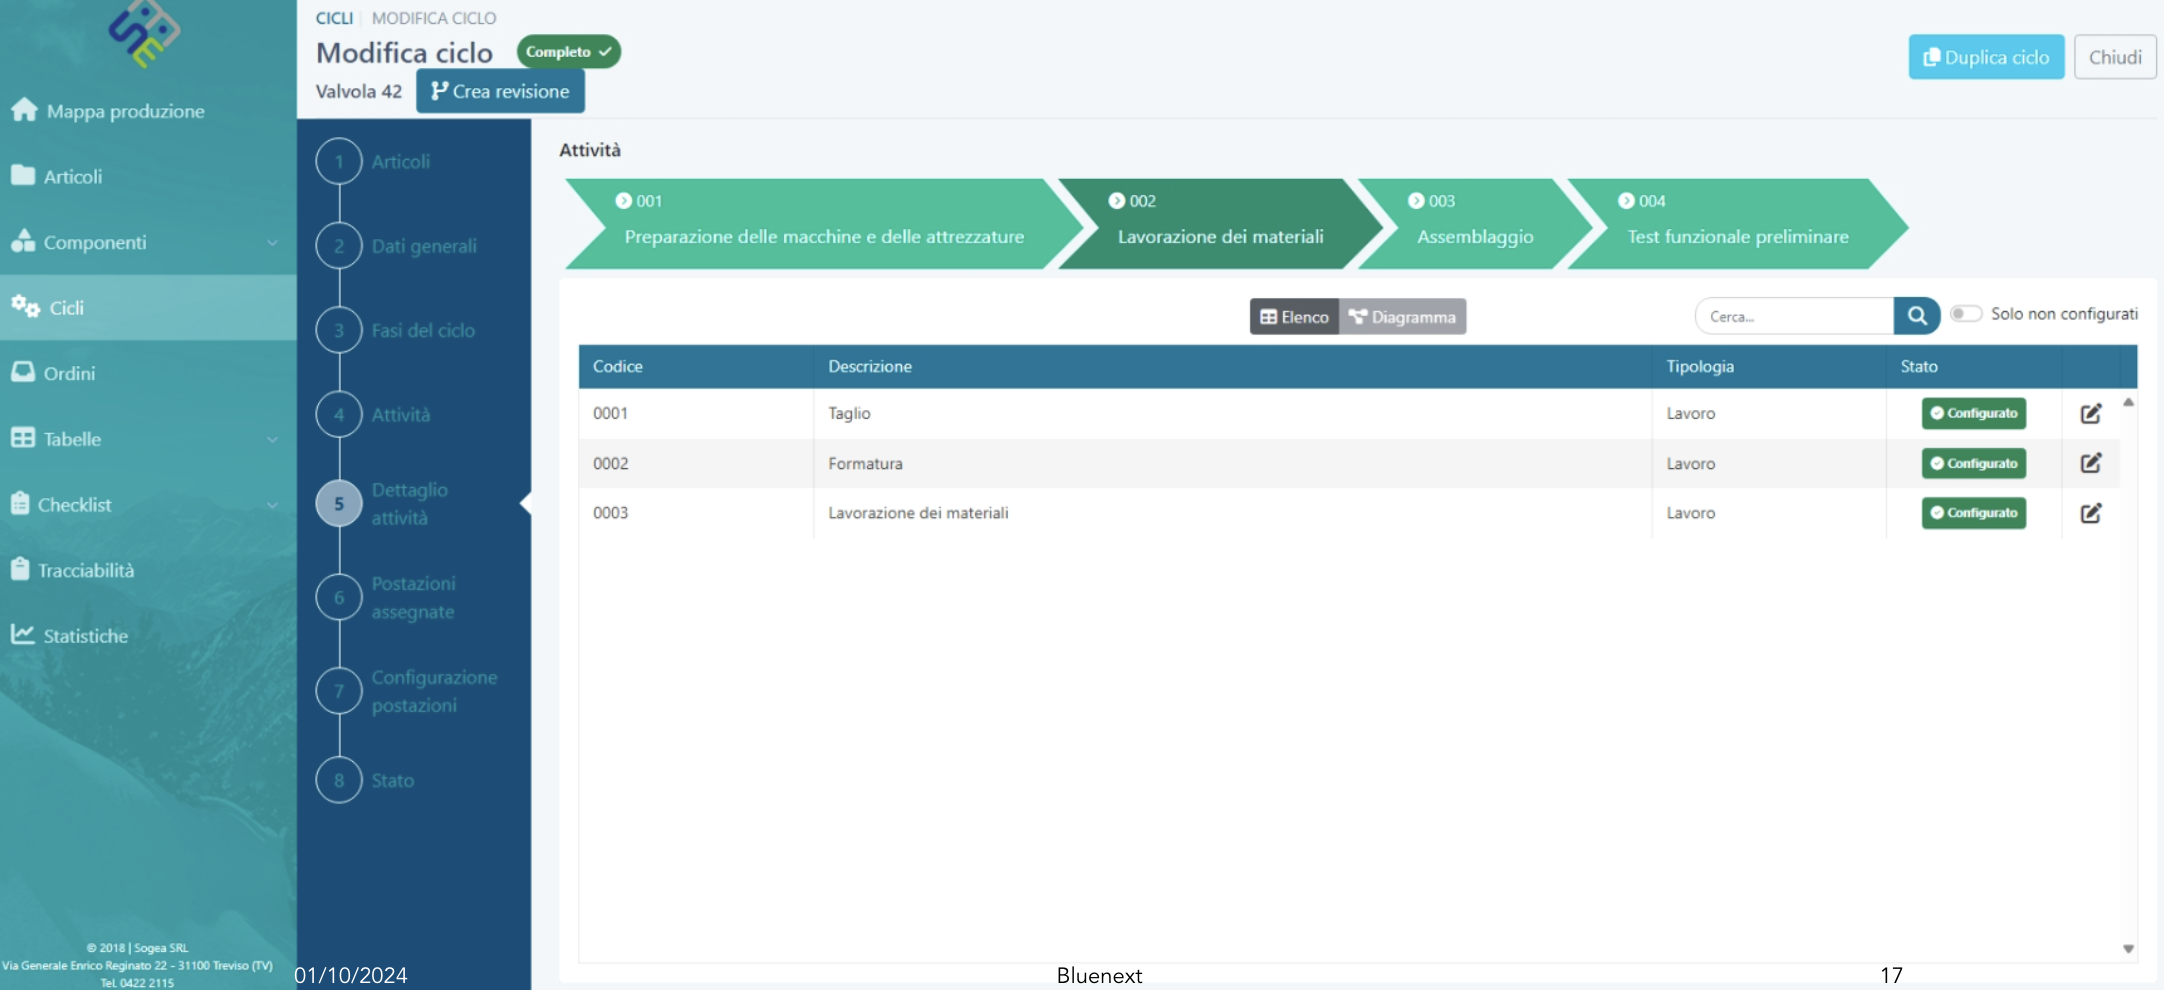
\includegraphics[width=1.0\linewidth]{BCS-Tessi//images/schermata_SAI.png}
            \caption[Schermata del \textit{software} SAI di SogeaSoft S.r.l.]{Schermata del \textit{software} SAI. Fonte: \textit{slide} di presentazione utilizzate durante la fase di formazione}
            \label{fig:screenSAI}
        \end{figure}
        
        \subsection{L'architettura di SAI}
        
            \subsubsection{Il monolite}
            
            Il \textit{software} SAI è caratterizzato da un’architettura monolitica, termine che evoca l’idea di una struttura compatta e unitaria, in cui le varie componenti sono strettamente interconnesse e formano un insieme indivisibile. Nel contesto dell'architettura \textit{software}, tale espressione indica un sistema in cui tutte le funzionalità sono integrate in un’unica unità di \textit{deployment}, costituendo una struttura unificata in cui ciascun componente dipende dagli altri per garantire il corretto funzionamento dell’intero sistema\footnote{O. Al-Debagy and P. Martinek, "A Comparative Review of Microservices and Monolithic Architectures," International Journal of Computer Science and Information Security, vol. 17, no. 3, pp. 123-131, 2019.}.  

            \vspace{0.2 em}
            \noindent Le principali caratteristiche di un’architettura monolitica sono le seguenti:  

            \begin{itemize}
                \item \textbf{integrazione delle funzionalità in un unico blocco applicativo}: tutte le funzionalità sono raccolte in un’unica entità, che viene distribuita come un blocco indivisibile. Questo implica che ogni modifica apportata a una parte del codice può avere ripercussioni su altre parti del sistema, rendendo complessi gli aggiornamenti e la manutenzione. Di conseguenza, con l’evolversi del progetto, l’accumulo di \text{debito tecnico\textsubscript{G}} può far sì che il \textit{software} diventi eccessivamente complesso e difficilmente adattabile a nuove tecnologie\footnote{J. Fritzsch, J. Bogner, A. Zimmermann, and S. Wagner, "From Monolith to Microservices: A Classification of Refactoring Approaches," in Proceedings of the IEEE International Conference on Software Architecture (ICSA), Stuttgart, Germany, 2018.};
                \item  \textbf{scalabilità verticale}: la scalabilità in un sistema monolitico si ottiene potenziando l’intera applicazione per affrontare un aumento del carico di lavoro. Anche qualora solo alcune funzionalità necessitassero di risorse aggiuntive, l’intero sistema deve essere aggiornato, comportando uno spreco di risorse. Non essendo possibile una scalabilità modulare, si tende a duplicare l’intera applicazione per garantire le prestazioni richieste;
                \item \textbf{bassa} \text{\textbf{granularità}\textsubscript{G}}: l’architettura monolitica presenta una scarsa separazione delle funzionalità, che risultano strettamente integrate e difficilmente isolabili\footnote{M. Cojocaru, A. Uta, and A.-M. Oprescu, "MicroValid: A Validation Framework for Automatically Decomposed Microservices," in Proceedings of the 11th IEEE/ACM International Conference on Cloud Computing (CloudCom), December 2019.}. Questo limita significativamente la flessibilità del sistema e ostacola l’integrazione di nuovi moduli o tecnologie senza compromettere la stabilità complessiva; 
            \end{itemize}  

            \vspace{0.2 em}
            \noindent L’architettura monolitica del sistema SAI rappresenta una sfida in termini di manutenibilità e adattabilità alle tecnologie moderne, evidenziando la necessità di migrare verso un’architettura a microservizi per migliorare la modularità, la scalabilità e l’agilità del sistema stesso.

            \vspace{0.2 em}
            \noindent L'obiettivo del mio \textit{stage} è quello di fornire una base formale e metodologica al lavoro empirico già avviato da SogeaSoft S.r.l. riguardo alla migrazione verso un'architettura a microservizi, con l’intento di superare i limiti strutturali del sistema attuale e di garantire una maggiore flessibilità e scalabilità in futuro. Una rappresentazione visuale di questa attività è visibile nella Figura 2.3.

            \subsubsection{I microservizi}
        
            L'architettura a microservizi si caratterizza per la natura decentralizzata e per l’unità di esecuzione non strettamente dipendente dalle altre componenti del sistema. I microservizi comunicano tra loro tramite reti di comunicazione, configurandosi come una forma di sistema distribuito. Un principio fondamentale di questa architettura è il \textit{$deploy_G$} indipendente, che si realizza garantendo un basso grado di accoppiamento (\textit{loose $coupling_G$}) tra i servizi\footnote{A. Makris, K. Tserpes, and T. Varvarigou, "Transition from monolithic to microservice-based applications: Challenges from the developer perspective," arXiv, vol. 1, 2020.}.  

            \vspace{0.2 em}
            \noindent Una caratteristica distintiva dei microservizi è l’assenza di un \textit{database} condiviso: ogni servizio mantiene il proprio \textit{database} locale e, qualora necessiti di accedere ai dati di un altro servizio, deve effettuare una richiesta esplicita. Questo approccio consente di definire con precisione quali dati sono visibili e quali rimangono nascosti, favorendo il \textit{deployment} indipendente\footnote{F. Hassan, "Software architecture between monolithic and microservices approach: Literature review," Department of Computer Science, University of Colorado, Boulder, CO, USA, 2020.}.  

            \vspace{0.2 em}
            \noindent Per garantire un’architettura efficace, i microservizi devono rispettare due principi fondamentali:  
            \begin{itemize}
                \item \textbf{Basso accoppiamento (\textit{Loose coupling})}: un microservizio è considerato debolmente accoppiato se è possibile modificarlo senza la necessità di aggiornare altri servizi correlati. Questo principio favorisce la manutenibilità e l'evoluzione del sistema, evitando effetti a cascata.
                \item \textbf{Alta coesione funzionale (\textit{High $\textbf{cohesion}_G$})}: ogni microservizio dovrebbe avere un unico e ben definito scopo, raggruppando le funzionalità in modo tale da minimizzare le modifiche in punti distinti del sistema. 
            \end{itemize} 

            \vspace{0.2 em}
            \noindent Inoltre, secondo i principi del \textit{Domain-Driven Design} ogni microservizio dovrebbe:  
            \begin{itemize}
                \item Incapsulare il \textit{domain $knowledge_G$} dai clienti, concentrandosi sulla propria responsabilità specifica. 
                \item Definire l’architettura e i confini in base al rispettivo dominio anziché all’intero sistema, garantendo una chiara separazione delle responsabilità e una gestione modulare delle funzionalità\footnote{E. Evans, Domain-Driven Design: Tackling Complexity in the Heart of Software, Addison-Wesley, 2003}..
            \end{itemize}  

            \vspace{0.2 em}
            \noindent Questo approccio consente di costruire sistemi resilienti e scalabili, in cui l'evoluzione tecnologica può avvenire in modo graduale e senza compromettere l'integrità complessiva del sistema.

            \begin{figure}[H]
                \centering
                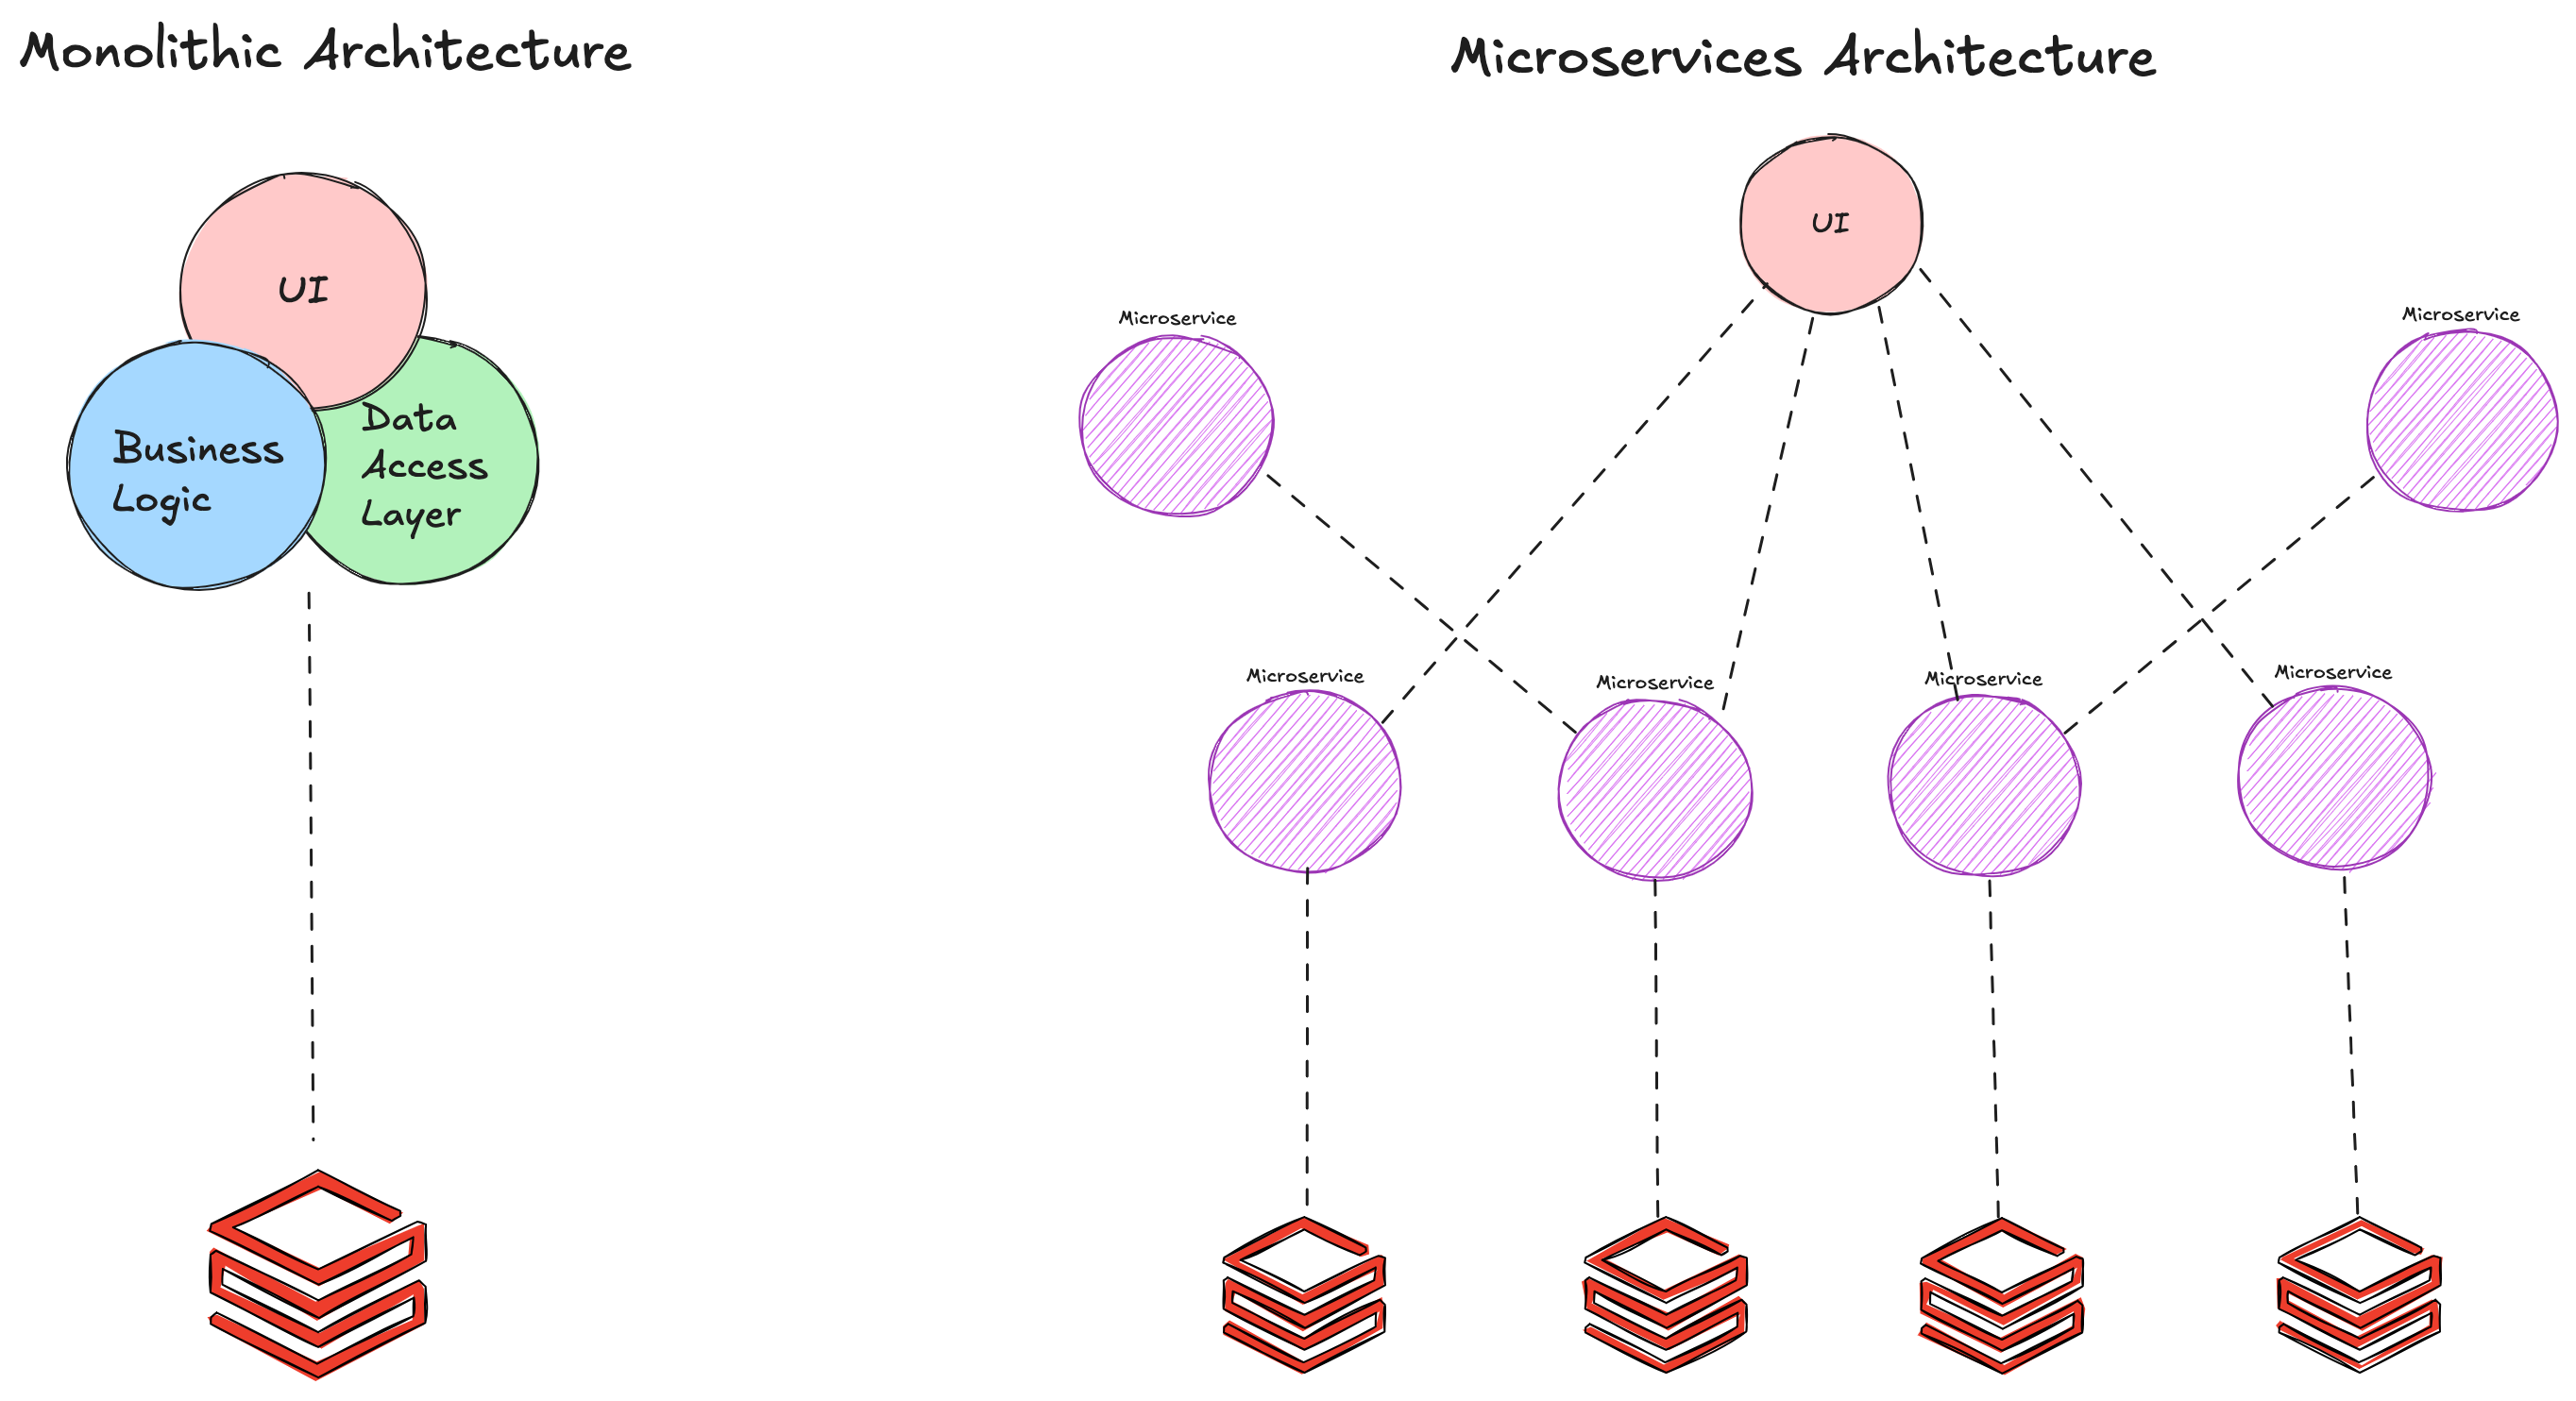
\includegraphics[width=1.0\linewidth]{BCS-Tessi/images/Monolith-Microservices.png}
                \caption[Differenza tra un sistema monolitico e uno a microservizi]{Differenza tra un'architettura monolitica e un'architettura basata su microservizi.}
                \label{fig:monolith-vs-microservices}
            \end{figure}

        \subsection{La migrazione}
        SogeaSoft S.r.l. desidera dunque migrare da un'architettura monolitica a un'architettura a microservizi. Già diverse attività sono state attuate a questo proposito e il mio compito è stato quello di porre una base teorica più solida ed eventualmente confermare o confutare le scelte implementate. Inoltre ho avuto l'occasione di partecipare ai processi decisionali riguardo a particolari casi d'uso nel mio progetto specifico di \textit{stage}. 
        SogeaSoft S.r.l. ha intrapreso un percorso di migrazione da un'architettura monolitica a un'architettura a microservizi, con l'obiettivo di migliorare la scalabilità, la manutenibilità e la flessibilità del proprio \textit{software} gestionale.  

        \vspace{0.2 em}
        \noindent Uno degli elementi centrali della migrazione riguarda l'introduzione di una componente denominata MicroService-Middleware, implementata come un \textit{Anti-Corruption $Layer_G$} ($ACL_G$). In ambito architetturale, un ACL è un modello progettuale che funge da interfaccia tra sistemi $legacy_G$ e nuove componenti, prevenendo la propagazione di modelli obsoleti o incoerenti nelle parti più moderne del sistema. Nel contesto di SogeaSoft S.r.l., il MicroService-Middleware si occupa di ricevere le richieste provenienti dall'ERP monolitico e, tramite un \textit{Message $Broker_G$}, instradare tali richieste verso il microservizio appropriato. Il \textit{Message Broker}, infatti, svolge il ruolo di intermediario per lo scambio di messaggi tra componenti \textit{software}, garantendo una comunicazione asincrona ed efficiente tra i vari microservizi.  

        \vspace{0.2 em}
        \noindent Ogni microservizio, una volta attivato, dopo aver effettuato l'autenticazione attraverso l'applicazione nativa di SAI chiamata \textit{Identity $Server_G$}, esso esegue la funzione richiesta in modo autonomo e indipendente, restituendo l’esito tramite lo stesso meccanismo di messaggistica. Per rendere accessibili le funzionalità esposte dai microservizi, l'azienda ha implementato una \textit{WebAPI Gateway}, che rappresenta un punto di accesso centralizzato alle API dei vari servizi. La \textit{WebAPI Gateway} consente di aggregare e orchestrare le chiamate ai microservizi, creando un'interfaccia unificata verso l'utente finale.  

        \vspace{0.2 em}
        \noindent Grazie a questa architettura, il sistema è in grado di supportare una \textit{Single Page $Application_G$} (SPA), un tipo di applicazione \textit{web} che carica una singola pagina \textit{web} e aggiorna dinamicamente il contenuto man mano che l'utente interagisce. Questo approccio garantisce un'esperienza utente più fluida e interattiva, riducendo i tempi di caricamento e ottimizzando le performance dell'applicazione.  

        \vspace{0.2 em}
        \noindent L'adozione di queste soluzioni riflette la volontà dell'azienda di superare le limitazioni dell'architettura monolitica, garantendo maggiore modularità e adattabilità alle nuove tecnologie, pur mantenendo la continuità dei servizi già in essere.

        \begin{figure}[H]
            \centering
            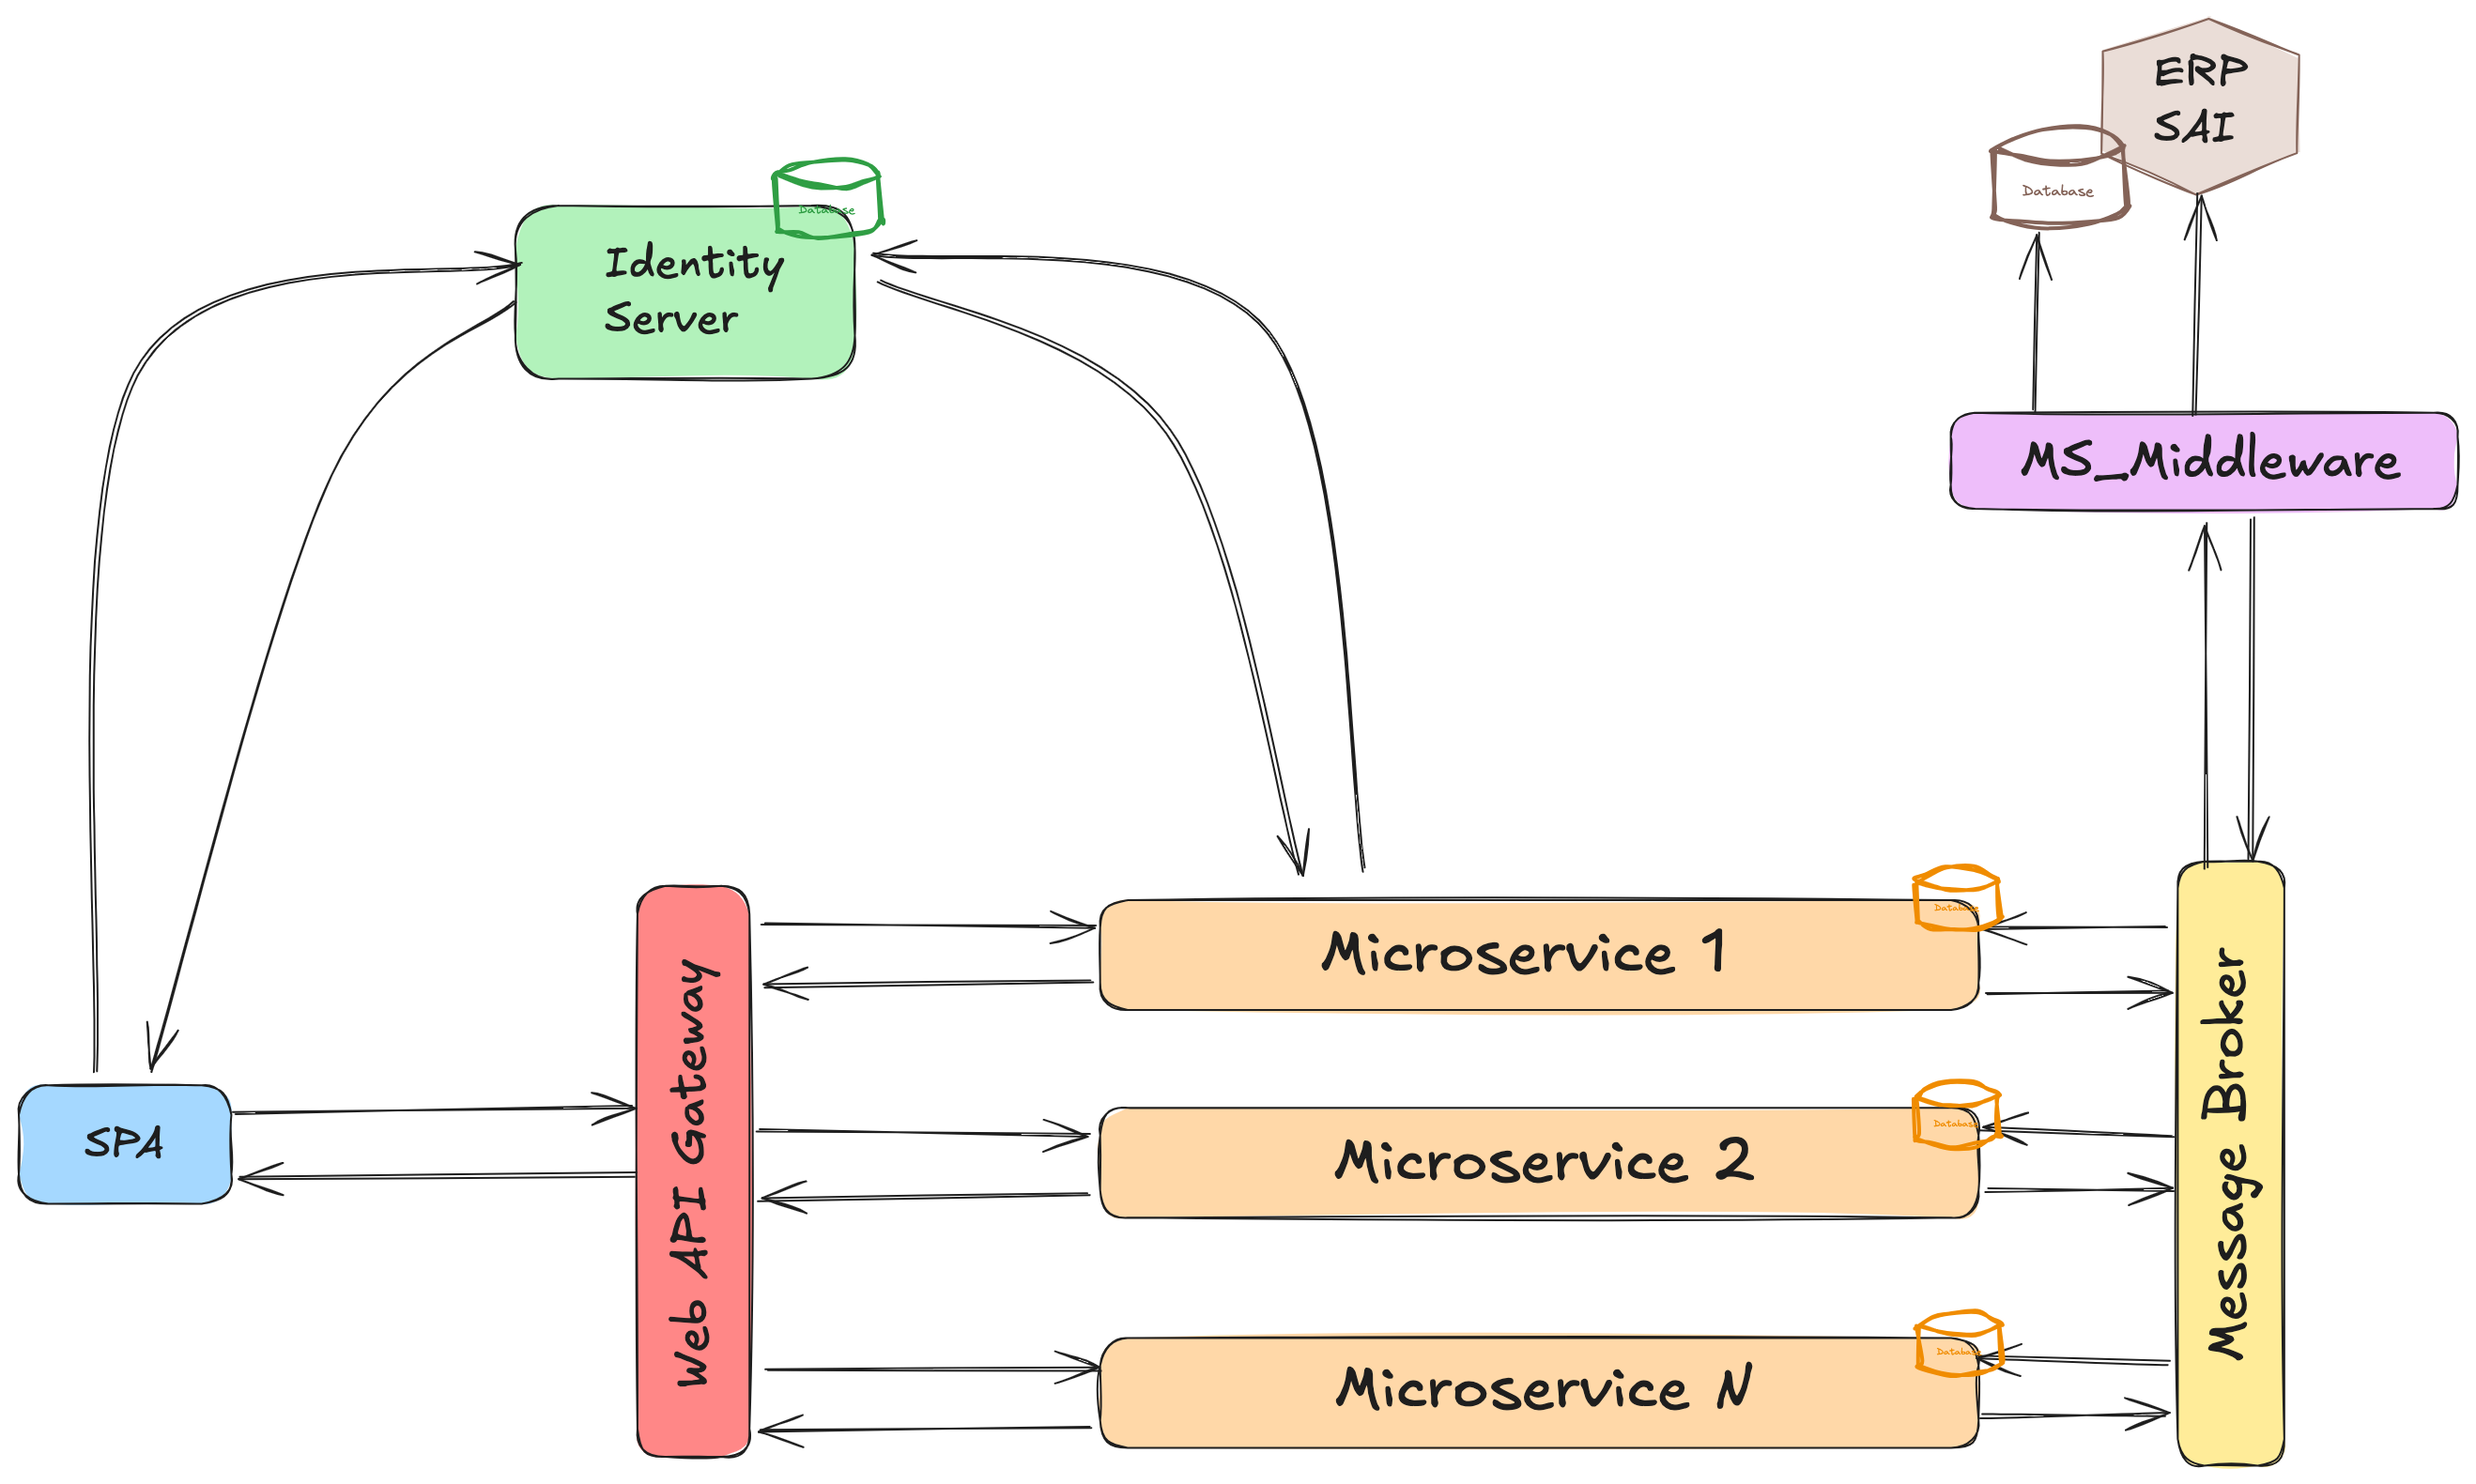
\includegraphics[width=0.6\linewidth]{BCS-Tessi/images/migrazione.png}
            \caption[Piano di migrazione di SogeaSoft S.r.l.]{Piano di migrazione di SogeaSoft S.r.l.. Fonte: informazioni apprese durante il processo di formazione. }
            \label{fig:enter-label}
        \end{figure}
        
    \section{Obiettivi del progetto di \textit{stage}}
        \subsection{Obiettivi aziendali}
        Nel contesto del mio progetto di \textit{stage}, SogeaSoft S.r.l. ha deciso di intraprendere un percorso di approfondimento riguardante la suddivisione del monolite in microservizi. Tale scelta si inserisce nell'ottica di favorire una maggiore modularità e flessibilità del sistema, nonché di facilitare futuri interventi di manutenzione e aggiornamento tecnologico.  

        Considerando che l’obiettivo dello stage è dimostrare concretamente le competenze acquisite, si è ritenuto opportuno effettuare l’estrazione di un microservizio come risultato tangibile dell’attività svolta. Questa operazione costituisce un esempio pratico del processo di migrazione verso un'architettura a microservizi e consente di valutare criticamente le scelte tecniche adottate.  

        A supporto dell’intero progetto, il tutor aziendale ha redatto un Piano di lavoro, un documento esaustivo che descrive l’azienda, gli obiettivi progettuali, i vincoli eventualmente presenti, la metodologia adottata e i risultati attesi. Tale documento costituisce un riferimento fondamentale per garantire la coerenza e la chiarezza delle attività intraprese durante lo stage. 

        \begin{table}[H]
        \centering
        \renewcommand{\arraystretch}{1.8} % Increase row height by 50%
        \begin{tabular}{|>{\bfseries}c|m{15cm}|} % Use 'm{}' for vertical centering
          \hline
          \multicolumn{2}{|c|}{\textbf{Obiettivi Aziendali}} \\ % First row, merged columns
          \hline
          \multicolumn{2}{|c|}{\textbf{Obbligatori}} \\ % Second row, merged columns
          \hline
          \multirow{2}{*}{\vspace*{\fill}OB1\vspace*{\fill}} & Studio della letteratura esistente sulle architetture monolitiche, sulle architetture a microservizi e sui metodi di migrazione \\ 
          \hline
          \multirow{2}{*}{\vspace*{\fill}OB2\vspace*{\fill}} & Documentazione relativa ai requsiti\\ 
          \hline
          \multirow{2}{*}{\vspace*{\fill}OB3\vspace*{\fill}} & Documentazione dei servizi esistenti e delle relazioni tra essi \\ 
          \hline
          \multirow{2}{*}{\vspace*{\fill}OB4\vspace*{\fill}} & Individuazione di un piano indicativo \\ 
          \hline
          \multicolumn{2}{|c|}{\textbf{Desiderabili}} \\ 
          \hline
          \multirow{2}{*}{\vspace*{\fill}DE1\vspace*{\fill}} & Documentazione dei rischi\\ 
          \hline
          \multicolumn{2}{|c|}{\textbf{Facoltativi}} \\ 
          \hline
          \multirow{2}{*}{\vspace*{\fill}FA1\vspace*{\fill}} & Realizzazione del PoC\\ 
          \hline
        \end{tabular}
        \caption[Descrizione degli obiettivi aziendali per il progetto di stage]{Descrizione degli obiettivi aziendali per il progetto di stage; corrispondono agli obiettivi redatti dal tutor aziendale nel Piano di lavoro.}
        \label{tab:obiettivi}
        \end{table}

        Gli obiettivi aziendali riportati nella Tabella ~\ref{tab:obiettivi} sono classificati secondo la seguente notazione:
        \begin{itemize}
            \item \textbf{Obiettivo obbligatorio (OB)}: rappresentano i requisiti obbligatori, vincolanti, che dovranno necessariamente essere soddisfatti;
            \item \textbf{Obiettivo desiderabile (DE)}: rappresentano i requsiti desiderabili, non vincolanti, ma dal riconoscibile valore aggiunto;
            \item \textbf{Obiettivo facoltativo (FA)}: rappresentano i requisiti facoltativi, rappresentanti di valore aggiunto ma non strettamente competitivo.
        \end{itemize}
        La rappresentazione tabellare utilizza la notazione [sigla][identificativo], dove la sigla indica la tipologia di obiettivo secondo la classificazione sopra descritta, mentre l’identificativo è un numero progressivo che garantisce l’univocità del requisito in combinazione con la sigla. 

        \subsection{Vincoli}
        
        Per quanto concerne i \textbf{vincoli temporali}, lo \textit{stage} curricolare deve svolgersi nell’arco di un monte ore compreso tra 300 e 320 ore, come previsto dal corso di studi, al fine di garantire un carico di lavoro equivalente a 12 crediti formativi universitari. Nel caso specifico del mio percorso formativo, tali ore sono state distribuite su un periodo di 8 settimane, con un impegno settimanale di 40 ore, articolate dal lunedì al venerdì, dalle ore 8:30 alle ore 17:00.   

        Per quanto riguarda i \textbf{vincoli tecnologici}, il piano di lavoro ha indicato i seguenti strumenti e metodologie:  
        \begin{itemize}
            \item Linguaggio di sviluppo: C\#;
            \item Ambiente di sviluppo: Visual Studio, Visual Studio Code;  
            \item Metodologia di sviluppo: Scrum (nell’ambito del framework \textit{Agile}) e $DevOps_G$, un insieme di pratiche e strumenti che integrano lo sviluppo software (Dev) e le operazioni (Ops) volte alla gestione delle infrastrutture tecnologiche. 
        \end{itemize}

        Tuttavia, nel corso dello \textit{stage} ho avuto l’opportunità di interagire anche con numerose altre tecnologie, che ho approfondito nella Sezione 1.7.

    \section{Metodo di Lavoro}
        \subsection{Piainificazione}
        
        Sulla base degli obiettivi di progetto delineati nella Sezione 2.3.1 (Tabella 2.1) e della pianificazione oraria proposta nel Piano di lavoro (Tabella 2.2), insieme al tutor aziendale, abbiamo stabilito le principali tappe intermedie (milestone) per monitorare il progresso del progetto. La collocazione temporale di queste milestone è stata determinata tenendo conto sia delle attività che dipendono strettamente l'una dall'altra, in particolare per quanto riguarda gli aspetti formativi, sia della necessità di produrre risultati tangibili, quali documentazione e codice, in modo regolare. Ciò ha permesso al tutor di monitorare il progresso del progetto e individuare tempestivamente eventuali rallentamenti.

        La definizione dettagliata delle singole attività è avvenuta nel corso delle sessioni di **sprint planning** con il Product Owner. Durante questi incontri, mi venivano assegnate le attività specifiche, venivano chiariti i risultati attesi e venivano fissati appuntamenti per valutare il grado di avanzamento, fornire supporto in caso di difficoltà o testare i risultati raggiunti. 

        Le sessioni di **sprint planning**, **sprint grooming** o **raffinamento del backlog** si sono svolte con una cadenza variabile, determinata in modo intuitivo in base alle necessità specifiche dei task a me assegnati, e si sono adattate di volta in volta al contesto e agli obiettivi da raggiungere.

        \begin{table}[h!]
        \centering
        \renewcommand{\arraystretch}{1.8} % Increase row height by 50%
        \begin{tabular}{|>{\bfseries}c|m{15cm}|} % Use 'm{}' for vertical centering
          \hline
          \multirow{2}{*}{\vspace*{\fill}Durata in ore\vspace*{\fill}} & Descrizione attività \\ 
          \hline
          \multirow{2}{*}{\vspace*{\fill}16\vspace*{\fill}} & Conoscenza ambiente di lavoro e contesto\\ 
          \hline
          \multirow{2}{*}{\vspace*{\fill}32\vspace*{\fill}} & Studio della letteratura esistente sulle architetture monolitiche, sulle architetture a microservizi e sui metodi di migrazione\\ 
          \hline
          \multirow{2}{*}{\vspace*{\fill}24\vspace*{\fill}} & Analisi dell'applicazione esistente per identificare i servizi e le funzionalità da suddividere in microservizi\\ 
          \hline
          \multirow{2}{*}{\vspace*{\fill}16\vspace*{\fill}} & Stesura della documentazione relativa ai requisiti\\
          \hline
          \multirow{2}{*}{\vspace*{\fill}24\vspace*{\fill}} & Studio dell'architettura a microservizi già esistente e analisi dei possibili miglioramenti per facilitarne la migrazione\\
          \hline
          \multirow{2}{*}{\vspace*{\fill}32\vspace*{\fill}} & Identificazione dei servizi monolitici da decomporre e delle relazioni tra essi.\\
          \hline
          \multirow{2}{*}{\vspace*{\fill}24\vspace*{\fill}} & Documentazione dei servizi esistenti e delle relazioni tra essi e del piano\\
          \hline
          \multirow{2}{*}{\vspace*{\fill}16\vspace*{\fill}} & Identificazione dei potenziali rischi e delle sfide associate alla migrazione\\
          \hline
          \multirow{2}{*}{\vspace*{\fill}24\vspace*{\fill}} & Inizio dello sviluppo di un Proof of Concept\\
          \hline
          \multirow{2}{*}{\vspace*{\fill}16\vspace*{\fill}} & Documentazione dei rischi\\
          \hline
          \multirow{2}{*}{\vspace*{\fill}8\vspace*{\fill}} & Individuazione di un piano indicativo di migrazione\\
          \hline
          \multirow{2}{*}{\vspace*{\fill}24\vspace*{\fill}} & Proseguimento del Proof of Concept\\
          \hline
          \multirow{2}{*}{\vspace*{\fill}16\vspace*{\fill}} & Valutazione teorica dell'architettura\\
          \hline
          \multirow{2}{*}{\vspace*{\fill}32\vspace*{\fill}} & Revisione della documentazione e del Proof of Concept\\
          \hline
          \multicolumn{2}{|c|}{\textbf{304 ore totali}} \\ % First row, merged columns
          \hline
        \end{tabular}
        \caption{Ripartizione delle ore in base alle attività}
        \label{tab:pianificazione-ore}
        \end{table}
        
        \subsection{Modello di sviluppo}
        SogeaSoft S.r.l. adotta un modello di sviluppo Agile basato su Scrum, come approfondito nella Sezione 1.4. Tuttavia, durante il mio stage, non ho partecipato a tutte le cerimonie previste dal framework Scrum. In particolare, sebbene il Daily Scrum meeting si svolgesse quotidianamente con il mio tutor (che si alternava al Product Owner, a causa della disponibilità e delle necessità di ciascuno), il mio coinvolgimento nelle altre cerimonie è stato limitato. Infatti, ho partecipato esclusivamente allo sprint planning e alla sprint review, che non avevano una durata fissa, ma variavano a seconda dei task assegnati e della disponibilità del Product Owner. Nel complesso, il mio lavoro è stato principalmente solitario, con sviluppo individuale e il supporto del tutor limitato a momenti specifici, come durante le sprint review o quando necessario durante i Daily. Uno schema utile per visualizzare il processo che ha caratterizzato le attività di sviluppo durante il mio stage è visibile in Figura \ref{fig:sprint-effettivi}.

        \begin{figure}[H]
            \centering
            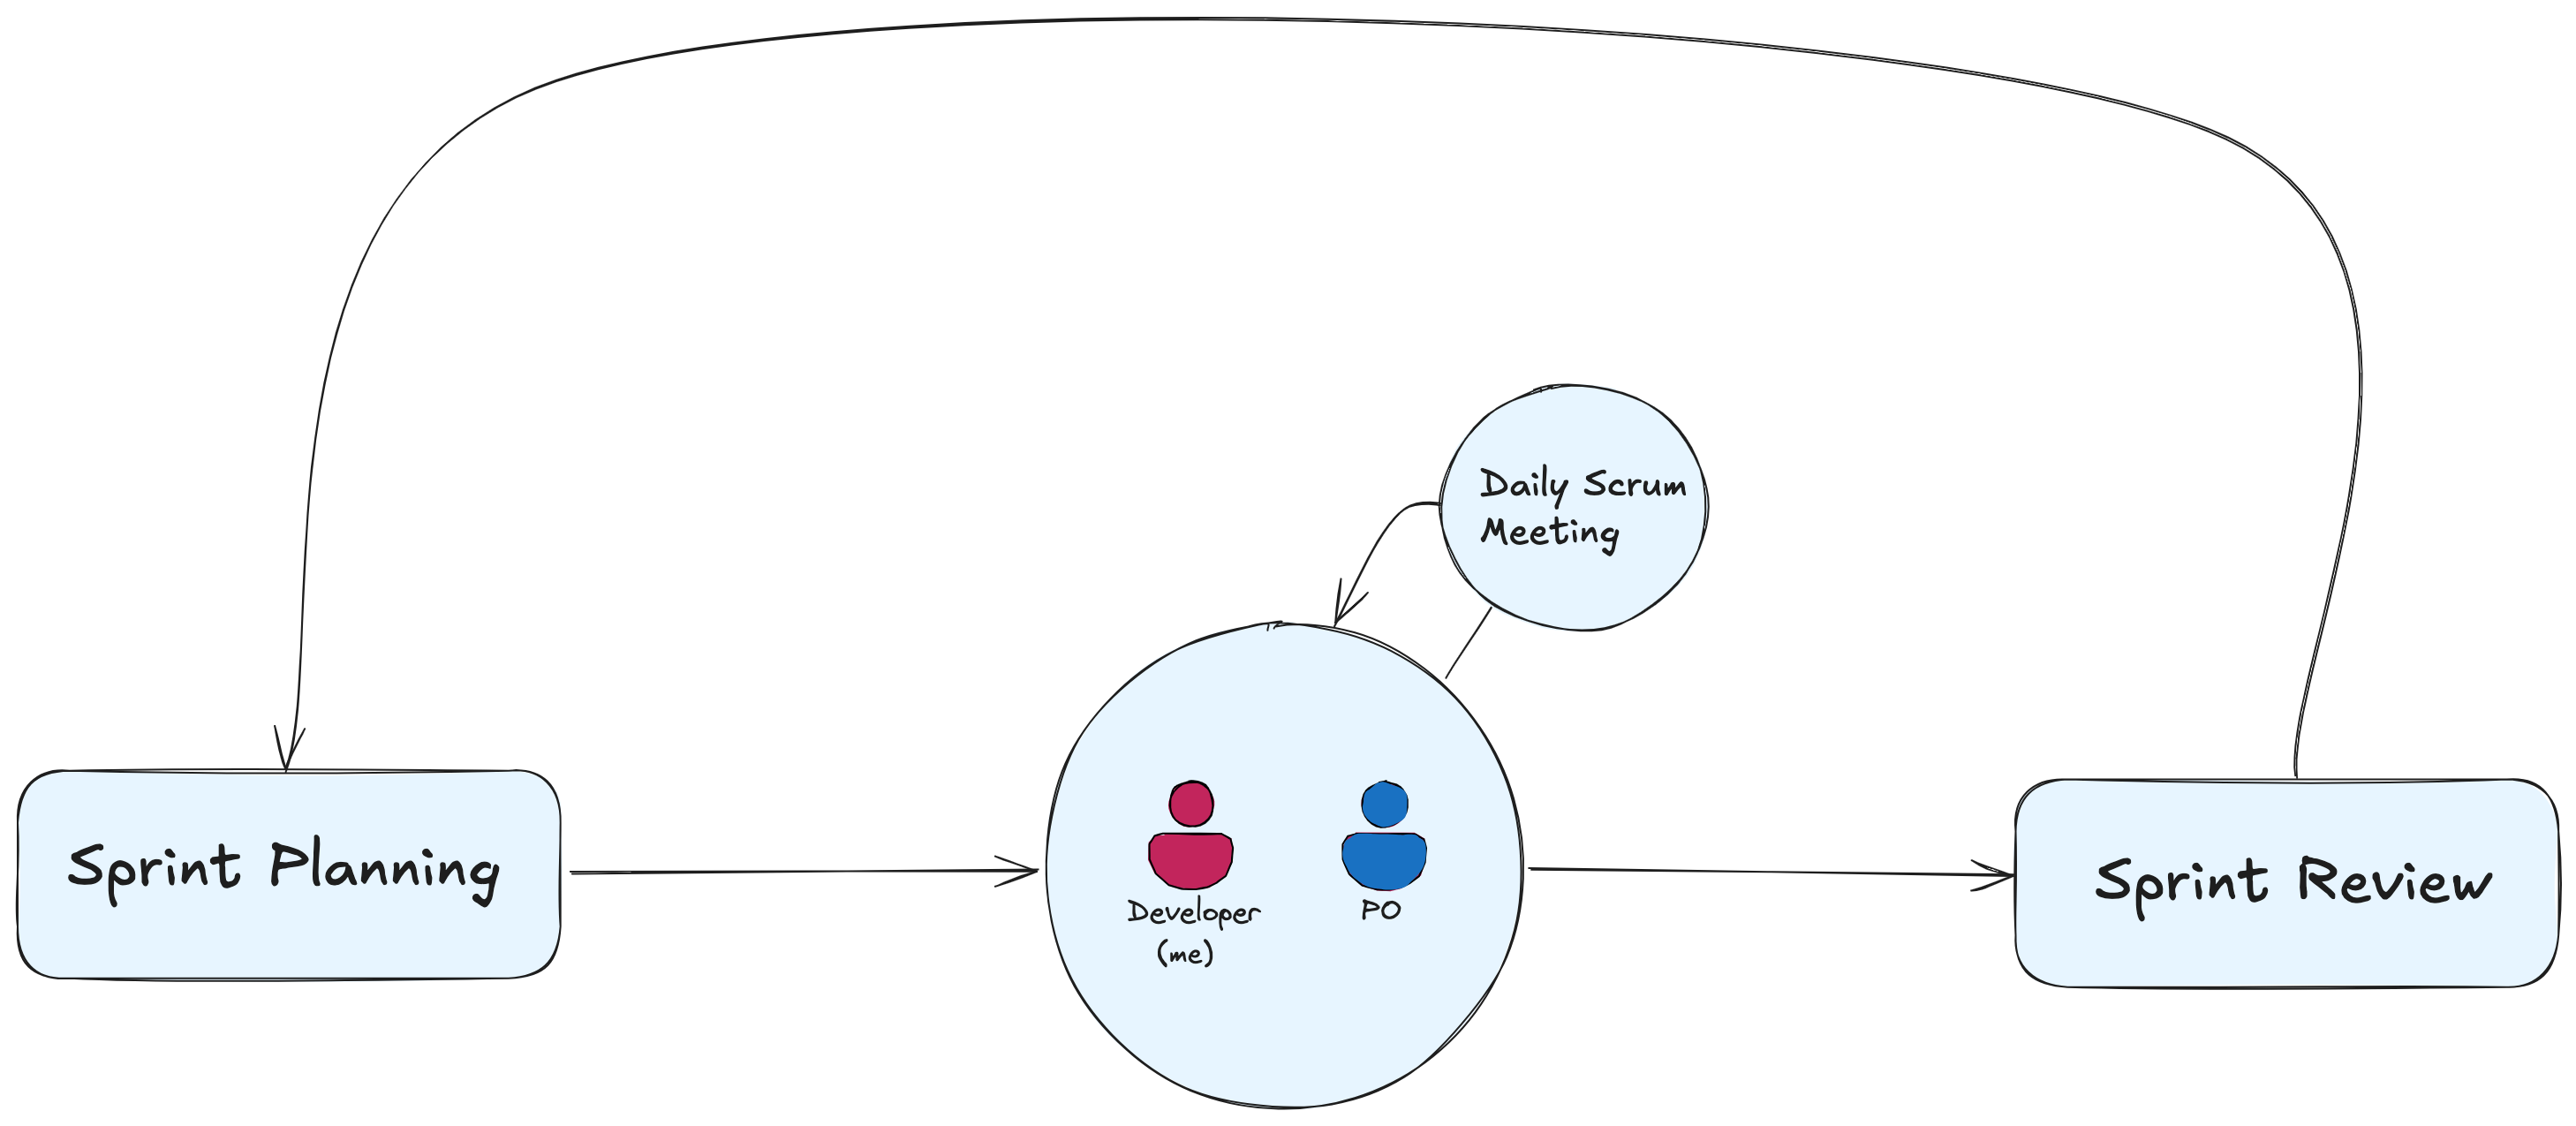
\includegraphics[width=0.7\linewidth]{BCS-Tessi/images/Sprint_true.png}
            \caption[Rappresentazione dell'attività di sviluppo effettiva secondo Agile (Scrum)]{Rappresentazione grafica dell'attività di sviluppo effettiva che ha caratterizzato il mio stage secondo Agile, nel contesto Scrum.}
            \label{fig:sprint-effettivi}
        \end{figure}
        
        \subsection{Strumenti}
        Gli strumenti utilizzati durante il mio stage, oltre alle tecnologie approfondite nella Sezione 1.7, sono stati diversificati e funzionali a diversi aspetti del lavoro. In primo luogo, ho impiegato la documentazione che redigevo progressivamente, utilizzando la Wiki di Azure come base di lavoro. Inoltre, per facilitare la gestione delle attività quotidiane e il processo di redazione della tesi, ho creato dei documenti personali in cui annotavo le cose da fare e le note importanti. 

        Ogni sessione di sprint planning è stata accompagnata dalla definizione dettagliata dei task da parte del Product Owner, al fine di evitare ambiguità nell’interpretazione delle attività. Questi task sono stati organizzati e conservati in una cartella Drive, dove ho anche archiviato libri, articoli e altre fonti utili trovate durante il progetto. 

        Poiché le pianificazioni erano gestite in modo intuitivo, non è stato necessario un ricorso frequente al calendario, in quanto il Product Owner mi comunicava direttamente le date degli incontri successivi. Un ulteriore strumento di monitoraggio utile è stato il report settimanale, che inviavo al mio tutor interno. Questi report mi hanno permesso di tracciare lo stato di avanzamento del progetto, identificare eventuali rallentamenti o problematiche, e di valutare se fosse opportuno rivedere le priorità tra le attività in corso.
        
        \subsection{Revisioni di Progresso}
        Riporterò tutte le occasioni di confronto con il \textit{tutor}, le revisioni ufficiali del lavoro svolto ed altri eventuali strumenti messi a disposizione per il monitoraggio del progresso. 
    \section{Motivazioni della scelta}
    Descriverò le motivazioni della mia personale scelta riguardo questo particolare progetto di \textit{stage}, raccontando perché l'ho scelto rispetto ad altri. Descriverò anche gli obiettivi e le aspettative personali, che riprenderò nella sezione 4.1.2
    
        